\documentclass[letterpaper]{article}
\usepackage[preprint]{aaai2027-course}
\usepackage[hyphens]{url}
\usepackage{graphicx}
\urlstyle{rm}
\def\UrlFont{\rm}
\usepackage{natbib}
\setcitestyle{numbers}
\usepackage{caption}
\usepackage{flafter}
\usepackage{stfloats}
\frenchspacing
\usepackage{algorithm}
\usepackage{algorithmic}
\usepackage{newfloat}
\usepackage{listings}
\DeclareCaptionStyle{ruled}{labelfont=normalfont,labelsep=colon,strut=off}
\lstset{basicstyle={\footnotesize\ttfamily},numbers=left,numberstyle=\footnotesize,xleftmargin=2em,aboveskip=0pt,belowskip=0pt,showstringspaces=false,tabsize=2,breaklines=true}
\floatstyle{ruled}
\newfloat{listing}{tb}{lst}{}
\floatname{listing}{Listing}
\usepackage{booktabs}
\usepackage{amsmath,amssymb}
\usepackage{array}
\usepackage{xeCJK}
\setCJKmainfont[AutoFakeBold=2.5]{Noto Serif CJK SC}
\setCJKsansfont[AutoFakeBold=2.5]{Noto Sans CJK SC}
\setCJKmonofont{Noto Sans Mono CJK SC}
\XeTeXlinebreaklocale "zh"
\XeTeXlinebreakskip = 0pt plus 1pt
\linespread{1.07}
\emergencystretch=2em
\setlength{\parskip}{0.08em plus 0.04em}
\setcounter{topnumber}{5}
\setcounter{bottomnumber}{5}
\setcounter{totalnumber}{10}
\setcounter{dbltopnumber}{5}
\renewcommand{\topfraction}{0.95}
\renewcommand{\bottomfraction}{0.9}
\renewcommand{\textfraction}{0.05}
\renewcommand{\floatpagefraction}{0.85}
\renewcommand{\dbltopfraction}{0.95}
\renewcommand{\dblfloatpagefraction}{0.85}
\setlength{\dbltextfloatsep}{0.55\baselineskip plus 0.2\baselineskip minus 0.15\baselineskip}
\setlength{\dblfloatsep}{0.5\baselineskip plus 0.2\baselineskip minus 0.15\baselineskip}
\setlength{\textfloatsep}{0.55\baselineskip plus 0.2\baselineskip minus 0.15\baselineskip}
\setlength{\floatsep}{0.5\baselineskip plus 0.2\baselineskip minus 0.15\baselineskip}
\setlength{\intextsep}{0.45\baselineskip plus 0.2\baselineskip minus 0.15\baselineskip}
\renewcommand{\abstractname}{摘要}
\renewcommand{\refname}{参考文献}
\setcounter{secnumdepth}{2}
\ifPDFTeX
\pdfinfo{
/TemplateVersion (2027.1-course)
}
\fi

\newcommand{\coursewidefigureplaced}[5][!tbp]{%
\begin{figure*}[#1]
\centering
\includegraphics[width=#2,height=#3,keepaspectratio]{#4}
\caption{#5}
\end{figure*}
}

\newcommand{\coursewidefigure}[4][0.94\textwidth]{%
\coursewidefigureplaced[!tbp]{#1}{#2}{#3}{#4}
}

\newenvironment{coursewidetable}[2][!tbp]{%
\begin{table*}[#1]
\centering
\small
\caption{#2}
\vspace{0.25em}
}{%
\end{table*}
}

\newenvironment{coursecolumntable}[1]{%
\begin{table}[H]
\centering
\footnotesize
\caption{#1}
\vspace{0.2em}
}{%
\end{table}
}

\title{基于多来源候选的文档扫描与增强系统}
\author{
    廖子杰 202534261067\\
    唐耿 202534261065
}
\affiliations{
    完成日期：2026年6月24日
}

\begin{document}
\pagestyle{empty}
\pagenumbering{gobble}

\maketitle

\begin{abstract}
尽管电子文档已经在现实世界普及，但是仍有很多打印的纸质文档，纸质文档的优势在于能够更加直观的阅读以及标记。
而在电子化时代，如何便捷的把纸质文档转换为电子版本仍是一个比较重要的课题。
在一般方案中，电子化往往由：1）文本扫描预处理，2）手写/打印文字识别，3）电子化归档这三个过程构成。
本文聚焦于文本扫描预处理这一过程，现有系统中，文档通常由人类手动拍摄，这会引入很多问题，如：
1）由于拍摄角度的限制，导致拍摄的图像存在倾斜等透视畸变
2）由于光照条件限制，被拍摄文档上光照不均，导致后续识别困难
3）部分文档可能存在折角或者缺损，使得对角点识别提出挑战
本项目着力于解决这一系列挑战，提出几个关键策略以及系统设计：
1）提出包含交点检测/面积合理性/宽高比合理性/直角程度等多因素加权四边形候选打分
2）提出基于高斯核的光照校正算法
3）构建了一套完整的识别处理系统，并开发了可用于实际使用的web页面
4）将构建的完整方法在MIDV以及DIBCO数据集上进行系统评估，着重对比一些非机器学习的传统方法
\end{abstract}

\begin{figure}[t]
\centering
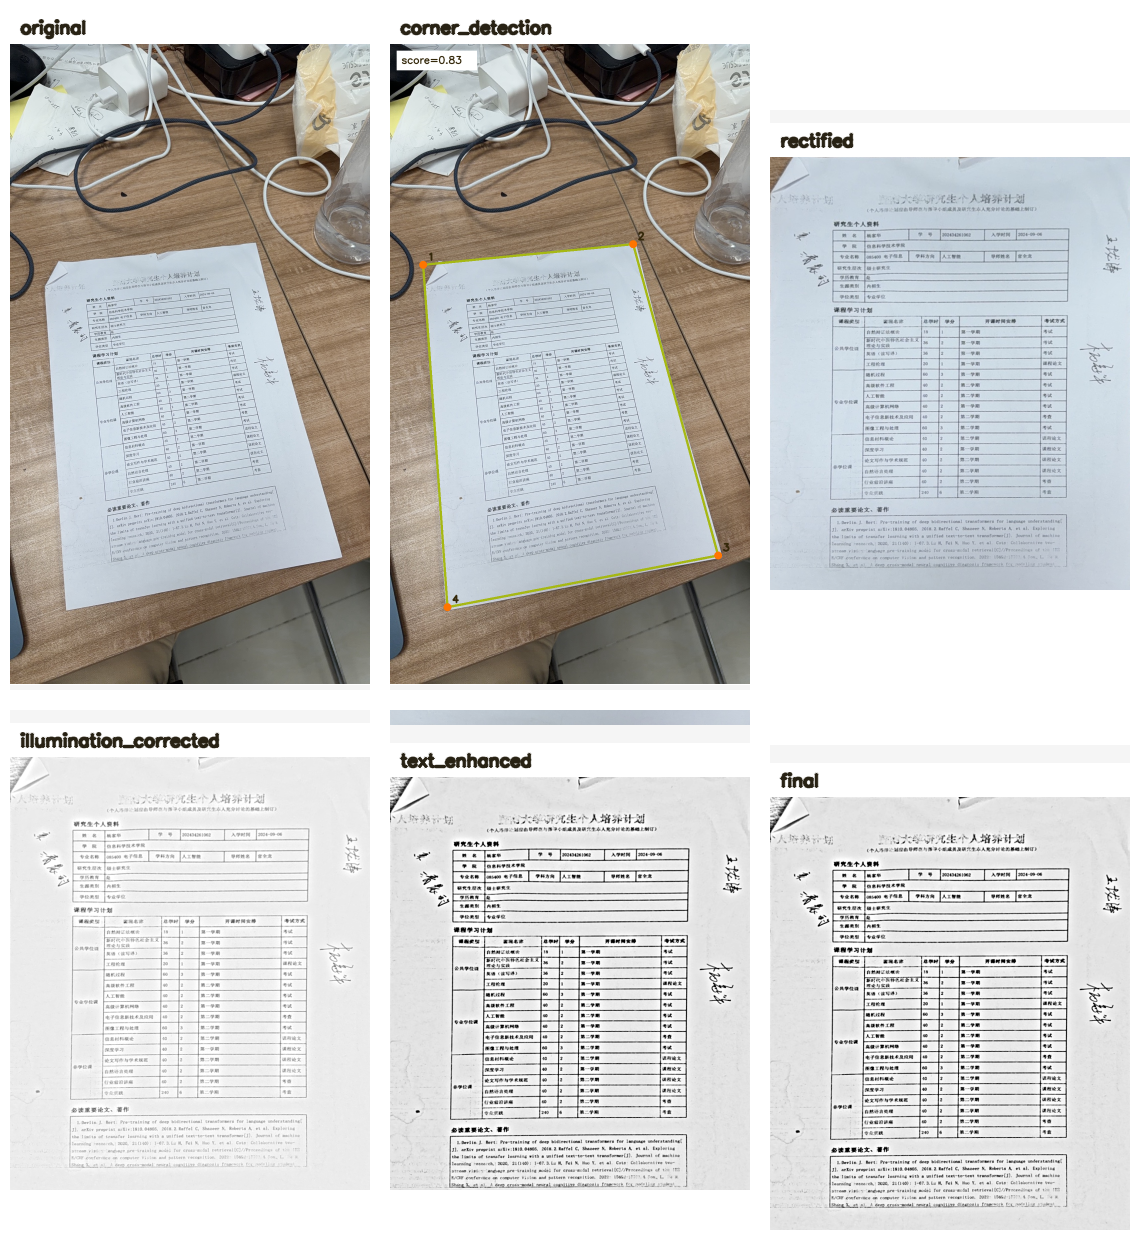
\includegraphics[width=0.9\columnwidth]{figures/pipeline_compact.png} 
\caption{复杂背景与折角场景下的核心处理链路：原图、角点检测、透视矫正、光照校正、文字增强和最终输出。}
\label{fig1}
\end{figure}

\section{算法原理与实现}

\subsection{方法总览}

单张图片会经过“输入预处理 $\rightarrow$ 角点定位 $\rightarrow$ 透视矫正 $\rightarrow$ 光照校正 $\rightarrow$ 文字增强 $\rightarrow$ 二值化对比 $\rightarrow$ 结果保存”。

流程：

\begin{enumerate}
\item 解码图片并缩放检测副本。
\item 灰度化、Gaussian blur、Canny 边缘检测。
\item 边缘连接与三路候选四边形生成。
\item 综合评分选择最优边界。
\item 四点单应性透视矫正。
\item 背景估计、光照归一化、低对比文字增强。
\item 输出多种二值化 artifact 和最终增强图。
\end{enumerate}

\subsection{角点定位}

为了完成具有鲁棒性的角点检测，我们实现了一个多候选融合方法，与以往只找最大轮廓的方法不同，我们的方法先生成多来源四边形候选，再用几何、边缘、纸面先验和局部修正共同确定最终四角点。

\subsubsection{输入与输出}

设输入图像为 $I$，输出文档四角点为：

\[
C=\{p_{tl},p_{tr},p_{br},p_{bl}\}
\]

为降低计算量，系统先将输入图像按最长边缩放到不超过 1000 px，得到检测图 \(I_d\)，并记录缩放比例 \(r\)。随后转灰度、Gaussian blur，再用 Canny 提取初始边缘：

\[
E_0 = \mathrm{Canny}(\mathrm{Gaussian}(Gray(I_d)))
\]

之后通过方形膨胀、闭运算、水平/垂直方向闭运算连接断裂边缘，得到增强边缘图 \(E\)。

\subsubsection{多来源四边形候选生成}

单一路径的四边形检测容易被真实拍摄中的强背景边缘、阴影、折角和局部遮挡干扰。因此系统不直接输出某一个轮廓，而是先生成候选四边形集合 \(\mathcal{Q}\)，再交给后续评分模块统一排序。设检测图尺寸为 \(W_d\times H_d\)，短边为 \(d=\min(W_d,H_d)\)。系统首先从 HSV 与 Lab 空间估计纸面似然：

\[
\begin{aligned}
L_p(x)={}&0.40\Big(1-\operatorname{clip}\frac{S(x)-35}{85}\Big)
\\
&+0.35\operatorname{clip}\frac{V(x)-125}{90}
+0.25\operatorname{clip}\frac{L(x)-135}{85},
\end{aligned}
\]

其中 \(S,V,L\) 分别表示饱和度、亮度和 Lab 明度，\(\operatorname{clip}(\cdot)\) 表示截断到 \([0,1]\)。在生成亮色区域候选时，还会构造二值纸面 mask：

\[
M_p=\big[S\leq\tau_s \land V\geq\tau_v \land L\geq\tau_l\big]
\lor \big[\operatorname{Otsu}(G)\land S\leq\tau_s\big],
\]

其中 \(\tau_v=\max(115,P_{62}(V))\)，\(\tau_l=\max(125,P_{58}(L))\)，\(\tau_s=\operatorname{clip}(P_{62}(S),45,105)\)，\(P_k\) 表示第 \(k\) 百分位数。这个 mask 不直接决定最终角点，而是作为纸面先验参与候选生成和候选评分，避免桌面边缘、阴影或整图边框被误认为文档边界。

最终候选集合由四类来源合并：

\[
\mathcal{Q}
=
\operatorname{Dedup}\big(
\mathcal{Q}_c\cup\mathcal{Q}_b\cup\mathcal{Q}_h\cup\mathcal{Q}_{lc}
\big).
\]

\textbf{轮廓候选 \(\mathcal{Q}_c\).}
系统在增强边缘图 \(E\) 上调用 \texttt{findContours}，按面积取前 48 个轮廓，并过滤面积小于 \(0.015W_dH_d\) 的噪声轮廓。对每个轮廓 \(\Gamma\)，同时考虑原始轮廓和凸包 \(H(\Gamma)\)。设轮廓周长为 \(P(\Gamma)\)，系统用多组精度
\(\epsilon\in\{0.008,0.012,0.016,0.02,0.03,0.045,0.06,0.08\}\)
执行 \texttt{approxPolyDP}：

\[
\hat{\Gamma}_{\epsilon}=\operatorname{approxPolyDP}(\Gamma,\epsilon P(\Gamma)).
\]

如果 \(\hat{\Gamma}_{\epsilon}\) 正好有 4 个点，则直接作为候选；如果其顶点数在 5 到 16 之间，则用极值点构造四边形：

\[
\begin{aligned}
p_{tl}&=\arg\min_{p\in\hat{\Gamma}}(x_p+y_p),&
p_{tr}&=\arg\min_{p\in\hat{\Gamma}}(y_p-x_p),\\
p_{br}&=\arg\max_{p\in\hat{\Gamma}}(x_p+y_p),&
p_{bl}&=\arg\max_{p\in\hat{\Gamma}}(y_p-x_p).
\end{aligned}
\]

此外，系统还加入 \texttt{minAreaRect} 的最小外接矩形作为补充候选。这一路适合边缘清晰的纸张，但在复杂桌面背景下容易被大背景轮廓误导。

\textbf{亮色区域候选 \(\mathcal{Q}_b\).}
对于白纸、证件和亮色文档，文档区域往往比背景更低饱和、更高亮。系统对 \(M_p\) 做多尺度形态学闭运算和开运算：开运算核大小约为 \(0.006d\)，闭运算核大小约为 \(0.010d,0.018d,0.030d\)。每个尺度产生一个候选 mask，并在其中寻找外部连通域。面积小于 \(0.04W_dH_d\) 的连通域会被丢弃，其余连通域复用轮廓候选中的 \texttt{approxPolyDP}、极值点和最小外接矩形生成四边形。这一路能够在 Canny 边缘断裂时提供稳定候选，但如果背景同样是浅色平面，就必须依赖后续纸面边界和边缘覆盖评分压低误检。

\textbf{Hough 长边候选 \(\mathcal{Q}_h\).}
当文档轮廓不闭合但四条直边仍然明显时，系统使用概率 Hough 变换检测长线段：

\[
\mathcal{L}=\operatorname{HoughLinesP}(E,\rho=1,\theta=1^\circ).
\]

阈值、最短线段和最大断裂间隔分别取
\(\max(70,0.09d)\)、\(\max(70,0.22d)\) 和 \(\max(20,0.05d)\)。检测出的线段按方向分为近水平和近垂直两类，再按位置聚类为上、下、左、右边。对任意满足间距约束的四组边线，
\[
y_{bottom}>y_{top}+0.18H_d,\quad
x_{right}>x_{left}+0.18W_d,
\]
系统求四条直线的交点得到候选四角。若直线写为 \(l=(a,b,c)\)，两个边界的交点可由齐次叉积得到：

\[
p_{ij}=l_i\times l_j.
\]

这一路对局部缺边更鲁棒，但单独使用时容易追随桌沿、屏幕边缘等长直线，因此更适合作为候选来源之一。

\textbf{低对比 Hough 兜底候选 \(\mathcal{Q}_{lc}\).}
如果前三类候选为空，或当前最高分低于 0.55，或最佳候选的边缘覆盖和四边覆盖都低于 0.12，系统会触发低对比兜底分支。该分支先用 CLAHE 增强灰度图，再用更低阈值 Canny 检测边缘：

\[
E_{lc}=\operatorname{Canny}(\operatorname{Gaussian}(\operatorname{CLAHE}(G)),25,75).
\]

随后使用更宽松的 Hough 参数生成线段，最短线段降到 \(\max(60,0.16d)\)，Hough 阈值降到 \(\max(50,0.07d)\)，并允许上下、左右边间距只需超过 \(0.12H_d\) 和 \(0.12W_d\)。候选会先用轻量几何分数排序：

\[
s_{lc}=0.45s_{angle}+0.35s_{area}+0.20s_{margin}-s_{border},
\]

最后最多保留前 64 个候选进入统一评分。这个分支牺牲一定精度来提高召回，主要用于投影、低光照和弱边缘场景。

所有来源生成的四边形都会执行同一组合法性约束。候选点先按左上、右上、右下、左下排序并裁剪到图像范围内；随后要求点坐标有限、四边形凸、面积比例满足

\[
0.055 \leq \frac{A(q)}{W_dH_d} \leq 0.98,
\]

且最短边长度不少于 \(0.08d\)。最后，系统会在 proposal 级和 candidate 级分别去重；若两个候选的平均角点距离小于 10 px，则只保留得分更高的候选。经过这一步后，\(\mathcal{Q}\) 中的每个元素都具有相同的几何格式和来源标签，可以交给下一节的综合评分函数比较。

\subsubsection{综合评分选择最优候选}

对每个候选 \(q\)，系统计算综合分数：

\[
\begin{aligned}
\operatorname{score}={}&
0.18a+0.16g+0.08ep+0.16sp\\
&+0.08c+0.06u+0.06m+0.04h+0.18p .
\end{aligned}
\]

其中 \(a,g,e,s,c,u,m,h,p\) 分别表示面积、角度、边缘覆盖、四边覆盖、内外亮度差、纸面平滑度、边距、长宽比和纸面边界支持。然后根据来源和贴近图像边界情况做小幅加减分，最后去重并取最高分候选。

\subsubsection{后处理}

选出初始最优候选后，还会进入后处理：

\begin{itemize}
\item 若候选来自 \texttt{low-contrast-hough}，系统会沿四条边的法线方向搜索局部边缘响应，用 Canny 支持和 Sobel 梯度拟合更贴近真实边界的边线；随后再尝试对四条边做小范围 offset 优化。
\item 其他来源会执行 \texttt{refine\_folded\_corners}：先在候选附近找到最大的纸面连通域，把其轮廓归一化到候选四边形坐标系中，在上下左右边附近重新拟合边线，再用边线交点替换可能落在折角或裁切内侧的角点。
\end{itemize}

最终角点是在检测尺度上得到，系统将角点除以缩放比例 \(r\)，映射回原图坐标，并裁剪到原图范围内：

\[
C_{orig}=C_d/r
\]

之后该角点集合会输入四点单应性透视变换，生成 \texttt{rectified} 文档正视图。

\subsection{透视矫正}

给定输入图像 \(I\)，角点定位阶段得到文档四角点：

\[
P=\{p_{tl},p_{tr},p_{br},p_{bl}\}
\]

其中四点按顺时针排序为：

\[
\begin{aligned}
p_{tl}&=(x_{tl},y_{tl}),&
p_{tr}&=(x_{tr},y_{tr}),\\
p_{br}&=(x_{br},y_{br}),&
p_{bl}&=(x_{bl},y_{bl})
\end{aligned}
\]

即左上、右上、右下、左下。

首先根据四边形上下边与左右边长度估计矫正后文档尺寸：

\[
W=\max(\|p_{br}-p_{bl}\|_2,\|p_{tr}-p_{tl}\|_2)
\]

\[
H=\max(\|p_{tr}-p_{br}\|_2,\|p_{tl}-p_{bl}\|_2)
\]

构造目标平面中的矩形顶点：

\[
Q=\{q_1,q_2,q_3,q_4\}
\]

其中：

\[
\begin{aligned}
q_1&=(0,0),&
q_2&=(W-1,0),\\
q_3&=(W-1,H-1),&
q_4&=(0,H-1)
\end{aligned}
\]

透视矫正的核心是求解从原图四边形到目标矩形的单应性矩阵 \(\mathbf{M}\)：

\[
s
\begin{bmatrix}
u\\
v\\
1
\end{bmatrix}
=
\mathbf{M}
\begin{bmatrix}
x\\
y\\
1
\end{bmatrix}
\]

其中 \((x,y)\) 是原图坐标，\((u,v)\) 是矫正后图像坐标，\(s\) 为齐次尺度因子，\(\mathbf{M}\) 为 \(3\times3\) 单应矩阵：

\[
\mathbf{M}=
\begin{bmatrix}
m_{11} & m_{12} & m_{13}\\
m_{21} & m_{22} & m_{23}\\
m_{31} & m_{32} & m_{33}
\end{bmatrix}
\]

对于每一组对应点 \(p_i \leftrightarrow q_i\)，有：

\[
u_i=\frac{m_{11}x_i+m_{12}y_i+m_{13}}
{m_{31}x_i+m_{32}y_i+m_{33}}
\]

\[
v_i=\frac{m_{21}x_i+m_{22}y_i+m_{23}}
{m_{31}x_i+m_{32}y_i+m_{33}}
\]

由四组点对应关系可建立 8 个线性约束，并在令 \(m_{33}=1\) 后求解单应性矩阵 \(\mathbf{M}\)。

获得 \(\mathbf{M}\) 后，对目标图像中的每个像素 \((u,v)\) 执行反向映射：

\[
s
\begin{bmatrix}
x\\
y\\
1
\end{bmatrix}
=
\mathbf{M}^{-1}
\begin{bmatrix}
u\\
v\\
1
\end{bmatrix}
\]

即：

\[
x=\frac{\hat{x}}{\hat{s}},\quad
y=\frac{\hat{y}}{\hat{s}}
\]

其中：

\[
\begin{bmatrix}
\hat{x}\\
\hat{y}\\
\hat{s}
\end{bmatrix}
=
\mathbf{M}^{-1}
\begin{bmatrix}
u\\
v\\
1
\end{bmatrix}
\]

最后使用插值方法从原图 \(I\) 中采样像素值，得到矫正图像：

\[
I_{rect}(u,v)=I(x,y)
\]

若 \((x,y)\) 不落在整数像素位置，则采用双线性插值：

\[
I(x,y)=
\sum_{i=0}^{1}\sum_{j=0}^{1}
w_{ij} I(x_i,y_j)
\]

其中 \(w_{ij}\) 由 \((x,y)\) 到相邻四个整数像素点的距离决定。

因此，完整透视矫正可概括为：

\[
I_{rect}=\mathcal{W}(I,P,Q,\mathbf{M})
\]

即通过四角点建立单应性变换，将原图中的任意透视四边形文档区域映射为正视矩形文档图像。

\subsection{光照矫正}

\textbf{光照校正方法}

给定透视矫正后的文档图像 \(I_{rect}\)，首先将其转换为灰度图：

\[
G(x,y)=Gray(I_{rect}(x,y))
\]

其中 \(G(x,y)\in[0,255]\)。

为了估计图像中的非均匀光照分布，使用大尺度高斯滤波得到背景光照图：

\[
B(x,y)=\mathcal{G}_{k\times k}(G)(x,y)
\]

其中高斯核大小 \(k\) 根据图像短边自适应确定：

\[
k=\mathrm{odd}\left(\mathrm{clip}(0.075\cdot \min(H,W),41,151)\right)
\]

为避免除零问题，对背景图进行下界约束：

\[
B(x,y)=\max(B(x,y),1)
\]

随后采用除法归一化消除慢变化光照：

\[
I_{c}(x,y)=\frac{G(x,y)}{B(x,y)}\cdot \alpha
\]

其中 \(\alpha\) 为亮度缩放系数，当前方法中取：

\[
\alpha=235
\]

因此，光照校正后的图像为：

\[
I_c(x,y)=\mathrm{clip}\left(235\cdot \frac{G(x,y)}{B(x,y)},0,255\right)
\]

该步骤的核心思想是将原始灰度图除以估计出的背景光照场，使阴影、亮斑等低频光照变化被抵消，而文字、边缘等高频结构被保留。

为了进一步保留暗色文字细节，计算背景图与原图之间的暗细节差分：

\[
D(x,y)=B(x,y)-G(x,y)
\]

并对其进行小尺度平滑：

\[
D_s(x,y)=\mathcal{G}_{3\times3}(D)(x,y)
\]

取暗细节图的高分位值作为全局细节强度：

\[
d_{high}=P_{99.3}(D_s)
\]

若 \(d_{high}>1\)，则计算自适应增强系数：

\[
\gamma=\mathrm{clip}\left(\frac{72}{d_{high}},1.35,5.0\right)
\]

否则：

\[
\gamma=0
\]

得到文字暗部增强项：

\[
T(x,y)=\mathrm{clip}(\gamma D_s(x,y),0,92)
\]

将该暗细节增强项从光照校正图中扣除，使文字区域进一步变暗、背景保持较亮：

\[
I_e(x,y)=I_c(x,y)-T(x,y)
\]

之后对增强图进行分位数拉伸。设：

\[
l=P_{0.7}(I_e),\quad h=P_{99.8}(I_e)
\]

则：

\[
I_s(x,y)=
\mathrm{clip}\left(
\frac{I_e(x,y)-l}{h-l}\cdot255,
0,255
\right)
\]

最后使用轻量锐化增强文字边缘：

\[
I_{sharp}=1.32I_s-0.32\mathcal{G}_{\sigma=0.75}(I_s)
\]

并通过边缘保持滤波抑制细小噪声，得到最终的光照校正与文字增强结果：

\[
I_{enhanced}=\operatorname{Bilateral}(I_{sharp})
\]

综上，光照校正过程可概括为：

\[
\begin{aligned}
I_{enhanced}
&=
\mathcal{F}\Bigg(
\mathrm{clip}\Big(
235\cdot\frac{G}{\mathcal{G}_{k\times k}(G)} \\
&\quad -
\gamma\big(\mathcal{G}_{3\times3}(\mathcal{G}_{k\times k}(G)-G)\big),
0,255
\Big)
\Bigg)
\end{aligned}
\]

其中 \(\mathcal{F}(\cdot)\) 表示分位数拉伸、轻量锐化和边缘保持平滑。该方法通过“背景光照估计 + 除法归一化 + 暗细节补偿”的方式，同时减弱阴影并增强低对比文字。

\subsection{文字增强}

给定灰度文档图像 \(G(x,y)\)、背景光照估计图 \(B(x,y)\) 以及光照校正图 \(I_c(x,y)\)，文字增强的目标是突出暗色笔画，同时尽量保持纸面背景平滑。

首先计算文档中的暗细节响应：

\[
D(x,y)=B(x,y)-G(x,y)
\]

其中 \(D(x,y)\) 越大，表示该位置相对于局部背景越暗，越可能属于文字笔画、印刷线条或图像细节。

对暗细节图进行小尺度平滑，抑制孤立噪声：

\[
D_s(x,y)=\mathcal{G}_{3\times3}(D)(x,y)
\]

随后利用高分位数估计整幅图中的文字细节强度：

\[
d_{high}=P_{99.3}(D_s)
\]

根据该强度自适应确定文字增强系数：

\[
\gamma=
\begin{cases}
\mathrm{clip}\left(\frac{72}{d_{high}},1.35,5.0\right), & d_{high}>1 \\
0, & d_{high}\leq 1
\end{cases}
\]

得到文字增强项：

\[
T(x,y)=\mathrm{clip}(\gamma D_s(x,y),0,92)
\]

由于文本通常表现为比背景更暗的区域，因此从光照校正图中扣除该增强项：

\[
I_t(x,y)=I_c(x,y)-T(x,y)
\]

该操作会进一步压低文字像素灰度，使文字与背景之间的对比度增大。

然后对增强图进行分位数拉伸。设：

\[
l=P_{0.7}(I_t),\quad h=P_{99.8}(I_t)
\]

则拉伸后的图像为：

\[
I_s(x,y)=
\mathrm{clip}
\left(
\frac{I_t(x,y)-l}{h-l}\cdot255,
0,255
\right)
\]

为了增强文字边缘，再进行反锐化处理：

\[
I_{u}(x,y)=
\lambda I_s(x,y)
-
(\lambda-1)\mathcal{G}_{\sigma}(I_s)(x,y)
\]

其中当前方法取：

\[
\lambda=1.32,\quad \sigma=0.75
\]

因此：

\[
I_u(x,y)=1.32I_s(x,y)-0.32\mathcal{G}_{0.75}(I_s)(x,y)
\]

最后使用边缘保持滤波抑制细小噪声，同时尽量保留文字边缘：

\[
I_{enhanced}=\operatorname{Bilateral}(I_u)
\]

此外，为了生成可读文字掩膜，计算相对暗度图：

\[
R(x,y)=
\frac{D_s(x,y)}{B(x,y)}\cdot255
\]

并对其进行平滑：

\[
R_s(x,y)=\mathcal{G}_{3\times3}(R)(x,y)
\]

通过 Otsu 阈值与前景比例约束共同确定文字阈值：

\[
\tau_{otsu}=\mathrm{Otsu}(R_s)
\]

\[
\tau_{ratio}=P_{88}(R_s)
\]

\[
\tau=
\mathrm{clip}
\left(
\max(6,\ 0.82\tau_{otsu},\ \tau_{ratio}),
6,\ 42
\right)
\]

得到初始文字掩膜：

\[
M(x,y)=
\begin{cases}
1, & R_s(x,y)>\tau \\
0, & R_s(x,y)\leq \tau
\end{cases}
\]

随后通过连通域面积约束去除过小噪点和过大非文字区域：

\[
M_f=\mathcal{C}(M)
\]

其中 \(\mathcal{C}(\cdot)\) 表示仅保留面积处于合理范围内的连通区域。

最终，可读文字二值图表示为：

\[
I_{bin}(x,y)=
\begin{cases}
0, & M_f(x,y)=1 \\
255, & M_f(x,y)=0
\end{cases}
\]

因此，文字增强过程可概括为：

\[
\begin{aligned}
I_{enhanced}
&=
\operatorname{Bilateral}\Big(
1.32\mathcal{S}(I_c-\gamma D_s) \\
&\quad -
0.32\mathcal{G}_{0.75}(\mathcal{S}(I_c-\gamma D_s))
\Big)
\end{aligned}
\]

其中 \(\mathcal{S}(\cdot)\) 表示分位数拉伸。该方法通过“暗细节估计、自适应增益、对比度拉伸、边缘锐化和连通域筛选”来增强低对比文档中的文字可读性。

\section{Web演示系统设计}

本系统采用前后端分离的 Web 演示架构，用于展示手机拍摄文档的扫描、矫正与增强过程。前端使用 \texttt{React + Vite + TypeScript} 实现移动端优先的实验验证界面，提供拍照上传、相册选择、参数调节、处理进度提示、中间结果网格和大图预览等功能；上传前会在浏览器端对大图进行压缩，以降低网络传输开销。

后端使用 \texttt{FastAPI + Pydantic} 提供轻量接口，核心接口为 \texttt{POST /api/scan}。前端以 \texttt{multipart/form-data} 上传图片和算法参数，后端完成图片校验、参数解析、图像处理、结果保存，并返回 \texttt{job\_id}、角点坐标、候选评分、性能指标和各阶段结果图 URL。中间结果以临时 PNG 文件形式存储，通过 \texttt{GET /api/results/\{job\_id\}/\{artifact\}} 读取。

图像处理部分基于上述章节描述的方法实现。如Figure~\ref{fig2}所示，整体流程包括：图像解码与缩放、灰度化与高斯滤波、Canny 边缘检测、形态学边缘连接、轮廓/亮色平面/Hough 线段三类候选四边形生成、综合评分选择文档边界、透视矫正、光照归一化、低对比文字增强，以及固定阈值、Otsu、Sauvola、Niblack、Wolf 等多种二值化结果对比。

\begin{figure}[t]
\centering
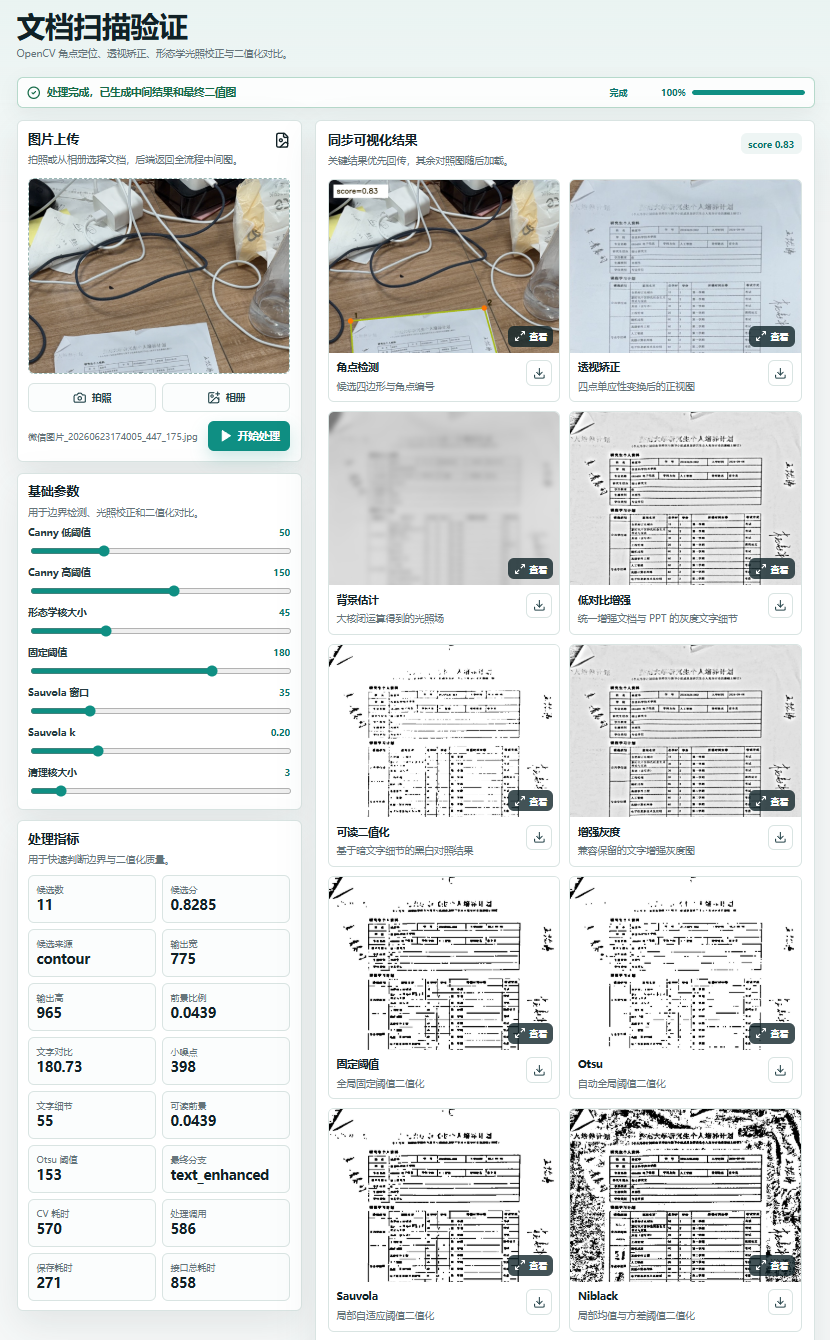
\includegraphics[width=0.4\textwidth]{figures/webui.png} 
\caption{实际的Web UI界面，该界面实现了上传图片到结果输出的完整流程展示}
\label{fig2}
\end{figure}


\section{实验设计与结果分析}

为了分别验证系统中的两个核心问题，本项目将实验分为几何定位实验和二值化增强实验。几何定位关注“能否在手机拍摄图像中准确找到文档四边形并完成透视矫正”，二值化增强关注“在已对齐的文档图像上，能否得到更接近人工标注的黑白文字结果”。因此本文没有把所有结果混合到同一张表中，而是针对不同数据集选择不同评价指标。

\subsection{数据集设置}

几何定位实验使用 MIDV-500 的局部样本。包含 3 类证件文档，每类覆盖 10 种拍摄条件，每个条件取 1 帧，共 30 张移动端拍摄图像。MIDV 提供每帧文档四边形标注，因此适合评价角点检测、文档边界定位和透视矫正的稳定性。该数据集包含桌面、键盘、手持、复杂背景和 partial 等不同条件，其中 partial 场景中文档可见区域较少，部分真实角点可能位于图像外，是当前算法的主要难点。

二值化实验使用DIBCO/H-DIBCO， 数据集提供了像素级前景/背景标注，适合评价二值化方法的准确率和失真程度。由于这些图像本身已经是文档内容图，不包含完整手机拍摄背景和外轮廓标注，因此本文不使用 DIBCO 评价角点定位。

\begin{coursecolumntable}{实验数据集与评价目标}
\resizebox{\columnwidth}{!}{%
\begin{tabular}{@{}llll@{}}
\toprule
数据集 & 数量 & 标注方式 & 主要用途 \\
\midrule
MIDV-500 & 30 & 四边形角点 & 几何鲁棒性评估 \\
DIBCO/H-DIBCO & 30 & 二值化 GT & 阈值与增强对比 \\
自建案例图 & 多个 & 无统一 GT & 中间过程展示 \\
\bottomrule
\end{tabular}%
}
\end{coursecolumntable}

\FloatBarrier

\subsection{评价指标}

针对 MIDV，本文将预测四边形 \(P\) 与真实四边形 \(G\) 都按左上、右上、右下、左下排序，并栅格化到原始图像尺寸上计算几何指标。四边形交并比定义为：

\[
\operatorname{IoU}(P,G)=
\frac{|M(P)\cap M(G)|}{|M(P)\cup M(G)|},
\]

其中 \(M(\cdot)\) 表示四边形在图像平面上的二值区域。Mean IoU 是所有样本 IoU 的算术平均，Median IoU 是中位数；由于 partial 场景中失败样本会显著拉低平均值，所以本文同时报告二者。角点平均误差按四个对应角点的欧氏距离计算：

\[
e_{corner}=\frac{1}{4}\sum_{i=1}^{4}\|p_i-g_i\|_2,
\qquad
e_{norm}=\frac{e_{corner}}{\sqrt{W^2+H^2}},
\]

其中 \(W,H\) 是原图宽高。表中的 \texttt{Mean corner err px} 即 \(e_{corner}\) 的平均值；\texttt{Corner <= 2\% diag} 表示 \(e_{norm}\leq0.02\) 的样本比例；\texttt{IoU >= 0.90} 表示 \(\operatorname{IoU}\geq0.90\) 的样本比例。Fallback rate 是候选生成失败、系统退回整图边界的比例。对于 partial 图像，还报告 GT 可见比例：

\[
r_{vis}=\frac{|M(G)\cap\Omega|}{|G|},
\]

其中 \(\Omega\) 表示图像可见区域，\(|G|\) 表示完整 GT 四边形面积；该值越低，说明真实文档越多部分位于画面外。

针对 DIBCO/H-DIBCO，本文先将 GT 与预测结果统一为黑色前景、白色背景，并统计像素级 \(TP,FP,FN,TN\)。Precision、Recall 和 F1 定义为：

\[
\begin{aligned}
P&=\operatorname{Precision}=\frac{TP}{TP+FP},\\
R&=\operatorname{Recall}=\frac{TP}{TP+FN},\\
F1&=\frac{2PR}{P+R}.
\end{aligned}
\]

pseudo-F1 使用 GT 前景骨架 \(S(G)\) 计算骨架召回：

\[
\begin{aligned}
R_{pseudo}&=\frac{|P_{fg}\cap S(G)|}{|S(G)|},\\
pseudo\text{-}F1&=\frac{2P R_{pseudo}}{P+R_{pseudo}},
\end{aligned}
\]

因此它更关注细笔画主体是否被召回。DRD 衡量误分类像素在局部邻域中的视觉失真。记误分类集合为 \(\mathcal{E}\)，5\(\times\)5 邻域权重为 \(w_{ij}\propto1/\sqrt{i^2+j^2}\)，并归一化到权重和为 1；则每个误分类像素的局部代价可写为：

\[
d(x)=\sum_{(i,j)\neq(0,0)}w_{ij}\,|G(x)-G(x+(i,j))|.
\]

最终 DRD 为：

\[
\operatorname{DRD}=\frac{\sum_{x\in\mathcal{E}}d(x)}{N_{UBN}},
\]

其中 \(N_{UBN}\) 是 GT 中非均匀 \(8\times8\) 图像块数量。DRD 越低，说明误分类越少出现在文字边界等视觉敏感区域。表中的 F1 最优次数表示某一方法在 30 张测试图中取得单图最高 F1 的次数。

\begin{coursewidetable}{MIDV-500 partial 样本的总体定位结果}
\small
\resizebox{\textwidth}{!}{%
\begin{tabular}{@{}lllllll@{}}
\toprule
范围 & Case & Mean IoU $\uparrow$ & Median IoU $\uparrow$ & IoU $\geq$ 0.90 $\uparrow$ & Corner $\leq$ 2\% diag $\uparrow$ & Fallback $\downarrow$ \\
\midrule
MIDV-500 partial & 30 & 0.6736 & 0.9328 & 53.33\% & 53.33\% & 0.00\% \\
\bottomrule
\end{tabular}%
}
\end{coursewidetable}

\begin{coursewidetable}{不同拍摄条件下的几何定位结果}
\small
\resizebox{\textwidth}{!}{%
\begin{tabular}{@{}lllllll@{}}
\toprule
条件 & Case & Median IoU $\uparrow$ & IoU $\geq$ 0.90 $\uparrow$ & Corner $\leq$ 2\% diag $\uparrow$ & Mean corner err px $\downarrow$ & 可见 GT 比例 \\
\midrule
\texttt{TS} & 3 & 0.9706 & 100.0\% & 100.0\% & 9.5 & 1.000 \\
\texttt{KS} & 3 & 0.9644 & 100.0\% & 100.0\% & 10.6 & 1.000 \\
\texttt{TA} & 3 & 0.9457 & 100.0\% & 100.0\% & 12.6 & 1.000 \\
\texttt{HA} & 3 & 0.9375 & 66.7\% & 66.7\% & 27.7 & 1.000 \\
\texttt{KA} & 3 & 0.9358 & 66.7\% & 66.7\% & 29.9 & 1.000 \\
\texttt{CA} & 3 & 0.9298 & 66.7\% & 66.7\% & 81.2 & 1.000 \\
\texttt{PA} & 3 & 0.5178 & 0.0\% & 0.0\% & 604.3 & 0.578 \\
\texttt{HS} & 3 & 0.4893 & 33.3\% & 33.3\% & 338.6 & 1.000 \\
\texttt{CS} & 3 & 0.4228 & 0.0\% & 0.0\% & 266.2 & 0.997 \\
\texttt{PS} & 3 & 0.0000 & 0.0\% & 0.0\% & 1078.7 & 0.216 \\
\bottomrule
\end{tabular}%
}
\end{coursewidetable}

\subsection{MIDV 角点定位与透视矫正结果}

在 30 张 MIDV-500 partial 样本上，当前完整方法取得了 0.9328 的 Median IoU，\texttt{IoU >= 0.90} 的成功率为 53.33\%，\texttt{Corner <= 2\% diag} 的成功率为 53.33\%，Fallback rate 为 0。这说明当前算法在多数正常可见文档场景中能够稳定给出文档四边形，但平均 IoU 被 partial 和复杂场景中的失败样本明显拉低。

从不同拍摄条件看，\texttt{TS}、\texttt{KS}、\texttt{TA} 等文档可见性较高、背景干扰较弱的场景表现最好，Median IoU 接近或超过 0.95；\texttt{CA}、\texttt{HA}、\texttt{KA} 等场景仍能保持较高的中位数表现；而 \texttt{PS}、\texttt{PA} 等 partial 场景明显困难，原因是目标文档只部分出现在画面中，GT 可见比例较低，真实角点可能在图像外，此时传统四边形候选更难稳定拟合真实边界。

为了验证综合评分策略的必要性，本文还比较了多种角点选择基准方法。结果显示，完整方法 \texttt{current\_full} 的 Median IoU 和高精度成功率优于只使用最大轮廓、最大面积、单一 Hough 长边或单一边缘得分的方法。\texttt{bright\_region\_score\_only} 的 Mean IoU 略高，说明亮色纸面先验很有效；但其 Median IoU 和 \texttt{IoU >= 0.90} 成功率低于完整方法，因此更适合作为候选来源之一，而不是替代综合评分。

\begin{coursewidetable}{角点候选选择策略消融对比}
\small
\resizebox{\textwidth}{!}{%
\begin{tabular}{@{}llllll@{}}
\toprule
角点方法 & Mean IoU $\uparrow$ & Median IoU $\uparrow$ & IoU $\geq$ 0.90 $\uparrow$ & Corner $\leq$ 2\% diag $\uparrow$ & Fallback $\downarrow$ \\
\midrule
\texttt{current\_full} & 0.6736 & 0.9328 & 53.33\% & 53.33\% & 0.00\% \\
\texttt{bright\_region\_score\_only} & 0.6947 & 0.9092 & 50.00\% & 50.00\% & 0.00\% \\
\texttt{current\_no\_refine} & 0.6676 & 0.9062 & 50.00\% & 53.33\% & 0.00\% \\
\texttt{contour\_score\_only} & 0.5927 & 0.8164 & 43.33\% & 43.33\% & 3.33\% \\
\texttt{largest\_contour} & 0.4571 & 0.4447 & 13.33\% & 16.67\% & 3.33\% \\
\texttt{max\_area} & 0.4287 & 0.3531 & 13.33\% & 13.33\% & 0.00\% \\
\texttt{hough\_lines\_score\_only} & 0.4053 & 0.3030 & 3.33\% & 16.67\% & 23.33\% \\
\bottomrule
\end{tabular}%
}
\end{coursewidetable}

该对比说明，文档边界检测不能简单依赖“最大轮廓”或“最大面积”。在真实手机拍摄图像中，桌面边缘、阴影、证件背景和图像边界都可能形成强轮廓，因此需要同时考虑面积、角度、边缘覆盖、四边支持、纸面亮度先验和边距惩罚等因素。完整方法相对 \texttt{current\_no\_refine} 的 Median IoU 从 0.9062 提升到 0.9328，也说明折角和局部边线修正对高精度定位有一定帮助。

\subsection{DIBCO/H-DIBCO 二值化方法对比}

在 DIBCO/H-DIBCO 的 30 张图像上，本文对固定阈值、Otsu、Sauvola、Niblack、Wolf、NICK、Bradley 以及本项目输出的 \texttt{binary\_readable}、\texttt{binary\_wolf\_fused} 进行对比。总体结果显示，\texttt{binary\_readable} 的平均 F1 最高，达到 0.6575；\texttt{binary\_nick} 的 pseudo-F1 最高，达到 0.6869；\texttt{binary\_bradley} 的 DRD 最低，说明其失真较小。本文实现的 \texttt{binary\_wolf\_fused} 相比普通 Wolf 方法有小幅提升，但当前默认最终输出仍选择保留灰度细节的 \texttt{text\_enhanced}，二值图主要作为对照和可读黑白输出。

分数据集来看，不同类型文档上的最优方法并不完全一致。DIBCO2019 Track A 上 \texttt{binary\_nick} 的 F1 最强，说明局部均值与方差对细笔画召回有优势；DIBCO2019 Track B 上 \texttt{binary\_otsu} 表现最好，说明在部分打印类、直方图分离较清晰的样本中，全局阈值仍有竞争力；H-DIBCO2018 手写文档上 \texttt{binary\_readable} 的 F1 最强，说明基于相对暗文字细节和连通域过滤的策略更适合低对比手写笔画。

因此，实验结论不是某一种二值化方法在所有场景下绝对最优，而是：当前系统保留多种二值化 artifact 是必要的。

\begin{coursewidetable}{DIBCO/H-DIBCO 二值化方法对比}
\small
\resizebox{0.8\textwidth}{!}{%
\begin{tabular}{@{}llllll@{}}
\toprule
方法 & 类型 & F1 $\uparrow$ & pseudo-F1 $\uparrow$ & DRD $\downarrow$ & F1 最优次数 \\
\midrule
\texttt{binary\_readable} & 当前可读二值图 & 0.6575 & 0.6765 & 3.2124 & 5 \\
\texttt{binary\_nick} & 局部阈值 & 0.6565 & 0.6869 & 2.4648 & 8 \\
\texttt{binary\_bradley} & 局部均值比例阈值 & 0.6377 & 0.6596 & 2.2828 & 5 \\
\texttt{binary\_wolf\_fused} & 本项目融合二值图 & 0.6287 & 0.6555 & 2.6526 & 3 \\
\texttt{binary\_wolf} & 局部阈值 & 0.6268 & 0.6536 & 2.6430 & 1 \\
\texttt{binary\_sauvola} & 局部自适应阈值 & 0.6009 & 0.5992 & 3.5048 & 4 \\
\texttt{binary\_fixed} & 固定全局阈值 & 0.5884 & 0.5852 & 3.6130 & 1 \\
\texttt{binary\_otsu} & 自动全局阈值 & 0.5659 & 0.5660 & 3.9732 & 3 \\
\bottomrule
\end{tabular}%
}
\end{coursewidetable}

\subsection{中间结果与最终输出展示}

定性结果主要展示算法链路是否可解释。图示案例包括原图、角点检测、透视矫正、背景估计、光照归一化、低对比增强、可读二值化和最终输出。如Figure~\ref{fig4}所示，原始图像存在复杂背景和折角，系统先定位文档区域，再通过透视变换得到正视图，随后进行光照校正和文字增强；以Figure~\ref{fig4}为例，可以观察到背景估计和除法归一化对阴影、投影和低对比文字的改善。

对于二值化对比，报告中保留代表性方法的精选对比图，展示不同阈值策略在噪声、细笔画保留和前景比例上的差异。角点检测图用于说明文档边界是否正确，\texttt{rectified} 用于说明透视矫正是否成功，\texttt{text\_enhanced} 用于说明阅读质量是否提升。

\begin{figure*}[t]
\centering
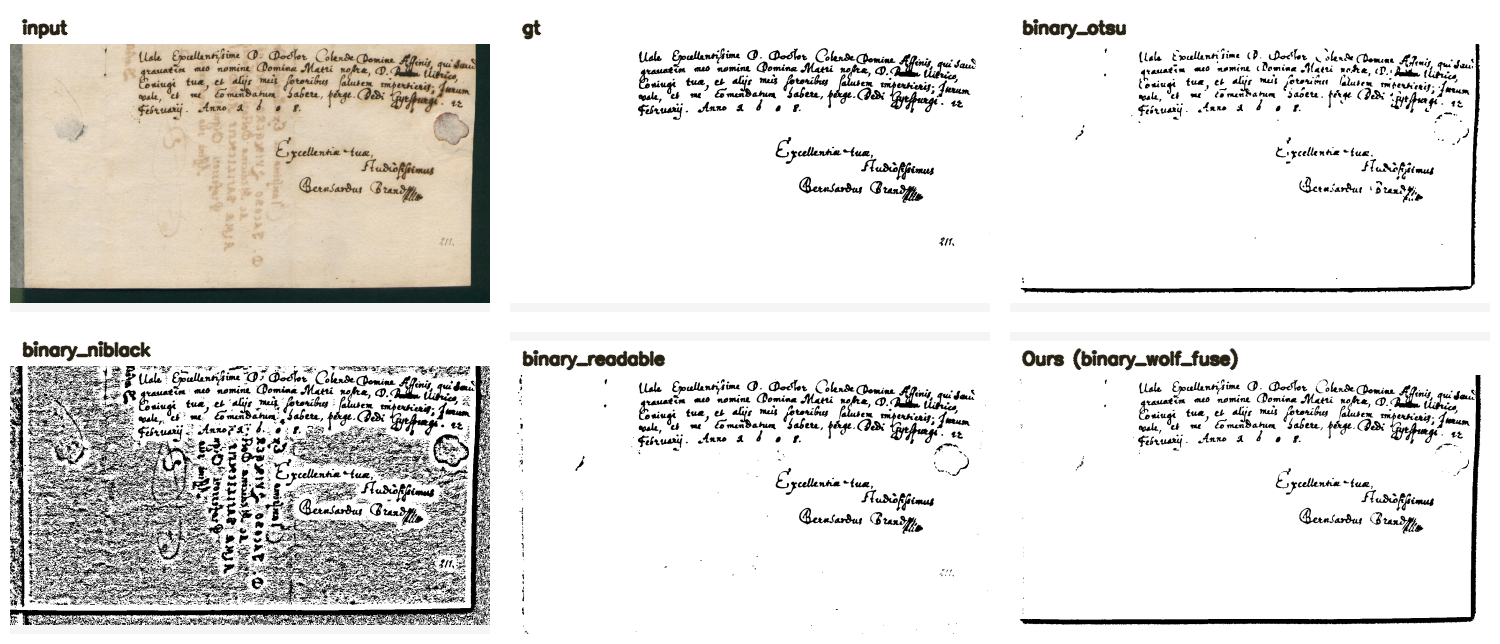
\includegraphics[width=0.9\textwidth]{figures/binarization_compact.png} 
\caption{二值化方法的定性对比：Niblack 易引入大量纹理噪声，Otsu 在部分样本上较干净，当前可读输出与融合结果更关注文字召回和可读性。}
\label{fig3}
\end{figure*}

\begin{figure}[t]
\centering
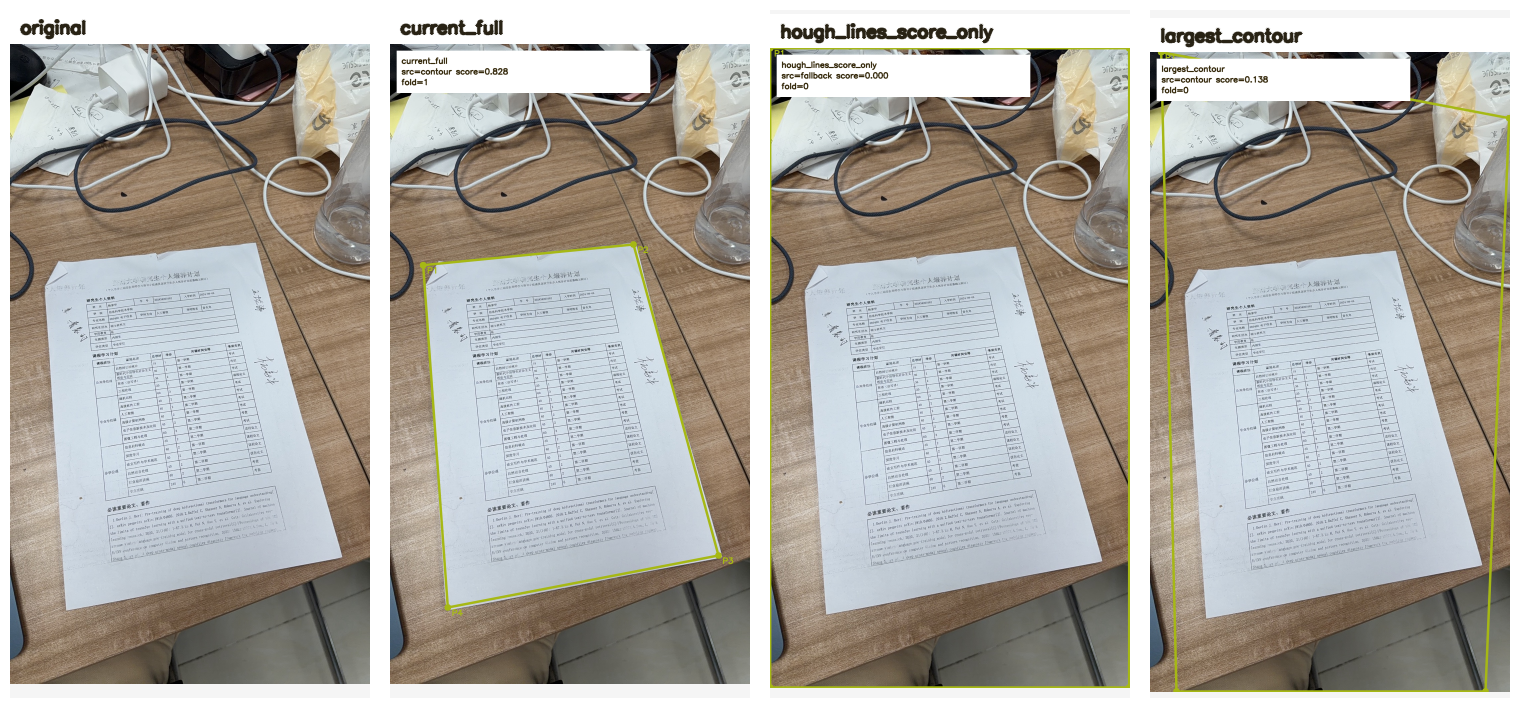
\includegraphics[width=0.9\columnwidth]{figures/corner_methods_row.png} 
\caption{角点定位方法的定性对比：完整方法能够贴合文档边界，而单一 Hough 或最大轮廓方法更容易被背景强边缘干扰。}
\label{fig4}
\end{figure}



\begin{figure}[t]
\centering
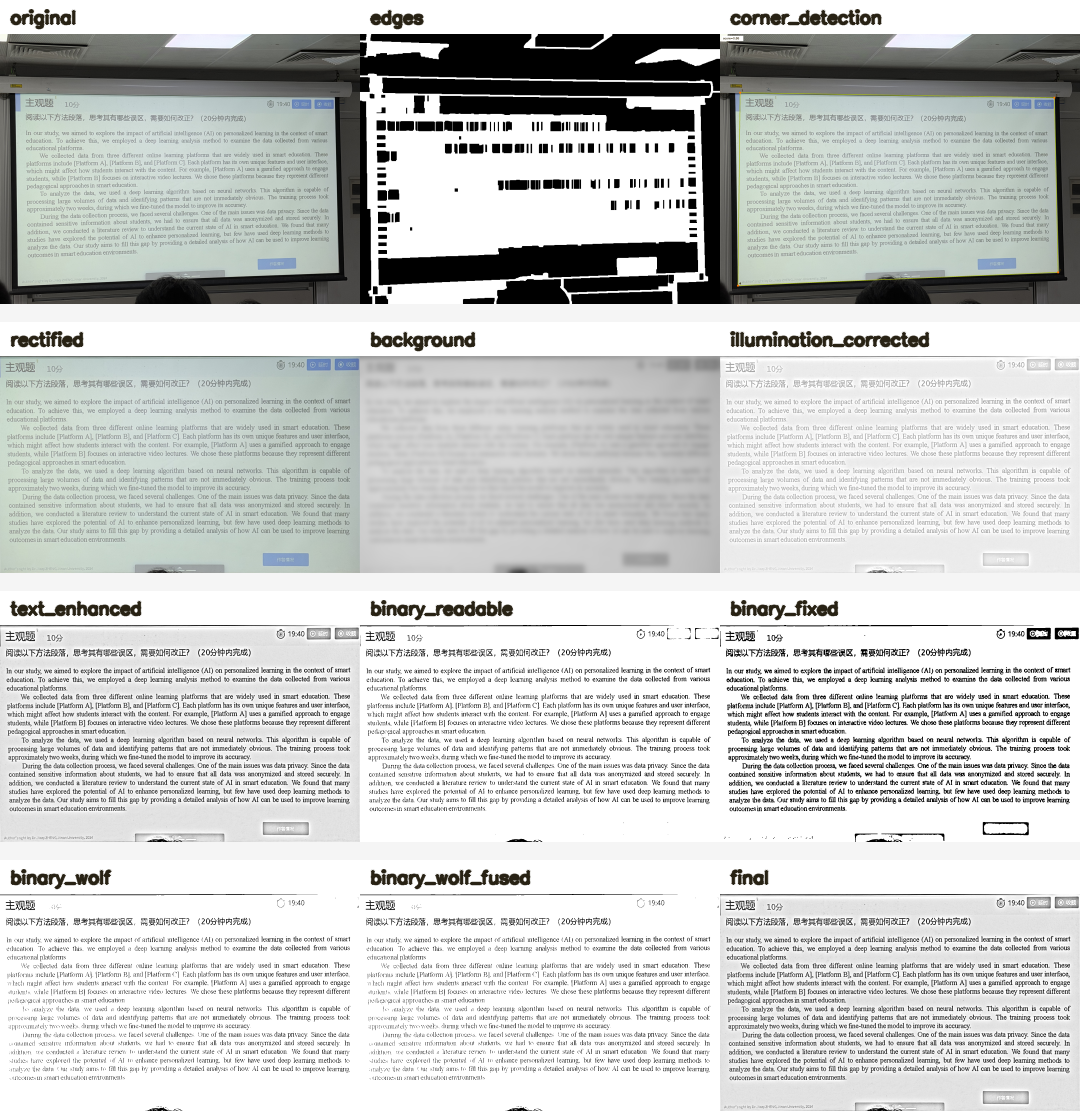
\includegraphics[width=0.9\columnwidth]{figures/case3_raw_pipeline_sheet.png} 
\caption{投影拍摄场景下的完整处理链路。背景估计与光照归一化能够削弱投影和低频光照变化，后续文字增强进一步提高阅读质量。}
\label{fig5}
\end{figure}

\section{结论与展望}

本项目的主要优点是可解释性强、部署轻量、过程可视化完整。算法不依赖深度学习模型，主要由 OpenCV 和 scikit-image 中的传统图像处理方法构成，因此每一步都有明确的中间结果和失败原因。MIDV 对比实验表明，多来源候选和综合评分比最大轮廓、最大面积等简单规则更稳定；DIBCO/H-DIBCO 实验表明，针对低对比文字设计的可读二值图在总体 F1 上优于固定阈值、Otsu 和 Sauvola 等经典基线。

当前方法的局限也比较明显。第一，部分极端场景仍然困难，当文档只露出一部分或真实角点位于图像外时，传统四边形模型难以准确表示目标边界，又或者低对比度场景，如白色桌面+白色文档的识别能力不足，具体见Figure~\ref{fig6}以及Figure~\ref{fig7}。第二，单应性透视变换假设文档近似平面，因此无法处理书页弯曲、纸张卷曲等非平面形变。第三，二值化结果在不同数据子集上没有统一最优方法，说明全局阈值、局部阈值和工程化增强各有适用场景。第四，当前 MIDV 实验是 30 帧轻量采样，不是完整 MIDV-500 benchmark，结果更适合作为课程项目中的可复现实验，而不是大规模公开榜单结论。

后续改进可以从三个方向展开：一是扩展 MIDV 样本数量，并增加课程场景自建数据集，对实验报告、试卷、书页等图像标注四角点，对方法添加更加针对性的评价；二是针对 partial 和强复杂背景场景增加更稳健的候选生成策略，例如边界延长、可见区域建模或轻量学习型边界检测；三是继续优化二值化融合策略，根据文档类型或图像统计特征自动选择更合适的输出，而不是固定使用单一阈值方法。

\begin{figure}[t]
\centering
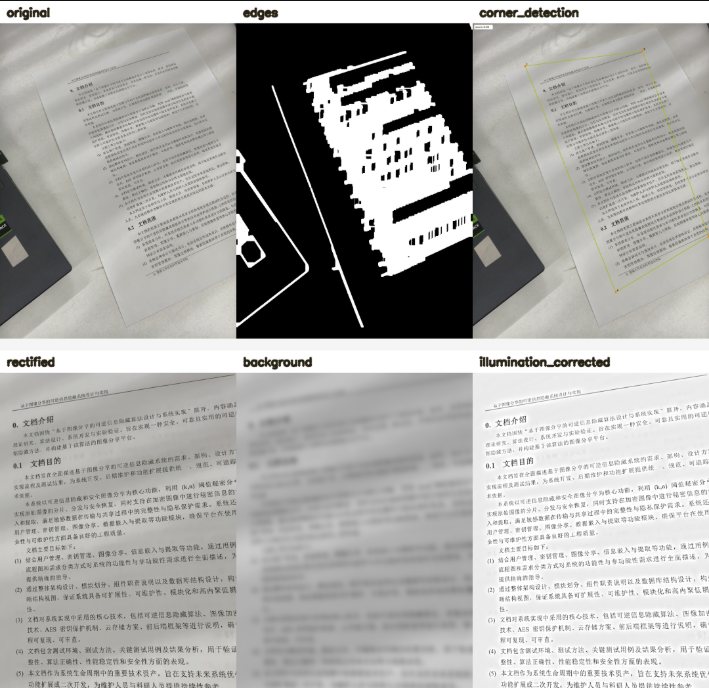
\includegraphics[width=0.9\columnwidth]{figures/bad_case1_pipeline_sheet.png} 
\caption{真实角点位于图像外时，模型难以准确表示目标边界}
\label{fig6}
\end{figure}

\begin{figure}[t]
\centering
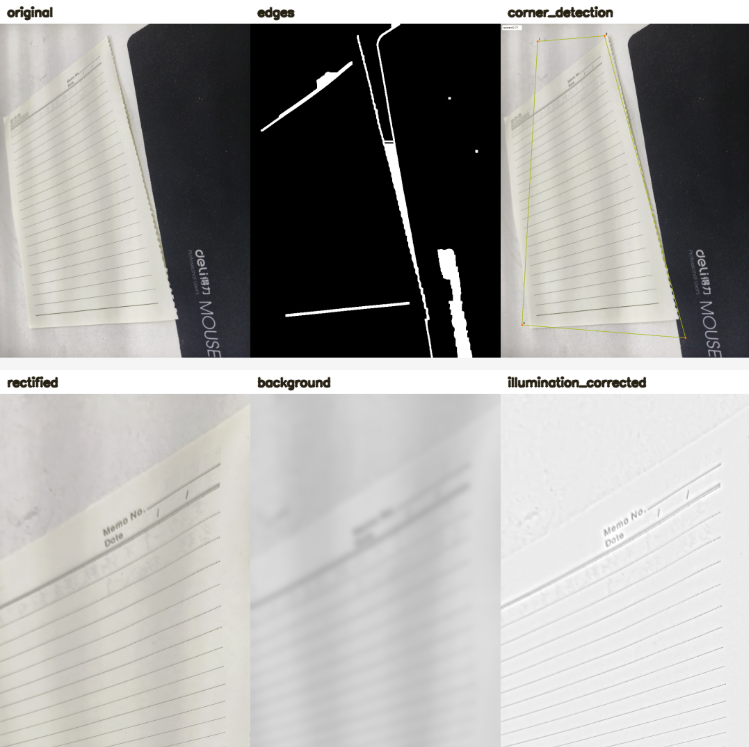
\includegraphics[width=0.9\columnwidth]{figures/bad_case2_pipeline_sheet.png} 
\caption{低对比度场景下的识别能力不足}
\label{fig7}
\end{figure}

\begin{thebibliography}{10}
\bibitem{ref1} Hartley R., Zisserman A. Multiple View Geometry in Computer Vision. 2nd ed. Cambridge University Press, 2004. DOI: \url{https://doi.org/10.1017/CBO9780511811685}
\bibitem{ref2} Canny J. A Computational Approach to Edge Detection. IEEE Transactions on Pattern Analysis and Machine Intelligence, PAMI-8(6): 679-698, 1986. DOI: \url{https://doi.org/10.1109/TPAMI.1986.4767851}
\bibitem{ref3} Duda R. O., Hart P. E. Use of the Hough Transformation to Detect Lines and Curves in Pictures. Communications of the ACM, 15(1): 11-15, 1972. DOI: \url{https://doi.org/10.1145/361237.361242}
\bibitem{ref4} Otsu N. A Threshold Selection Method from Gray-Level Histograms. IEEE Transactions on Systems, Man, and Cybernetics, 9(1): 62-66, 1979. DOI: \url{https://doi.org/10.1109/TSMC.1979.4310076}
\bibitem{ref5} Sauvola J., Pietikäinen M. Adaptive Document Image Binarization. Pattern Recognition, 33(2): 225-236, 2000. DOI: \url{https://doi.org/10.1016/S0031-3203(99})00055-2
\bibitem{ref6} Wolf C., Jolion J.-M., Chassaing F. Text Localization, Enhancement and Binarization in Multimedia Documents. Proceedings of the 16th International Conference on Pattern Recognition, 2: 1037-1040, 2002. DOI: \url{https://doi.org/10.1109/ICPR.2002.1048482}
\bibitem{ref7} Khurshid K., Siddiqi I., Faure C., Vincent N. Comparison of Niblack Inspired Binarization Methods for Ancient Documents. Document Recognition and Retrieval XVI, SPIE Proceedings, 7247: 72470U, 2009. DOI: \url{https://doi.org/10.1117/12.805827}
\bibitem{ref8} Bradley D., Roth G. Adaptive Thresholding Using the Integral Image. Journal of Graphics Tools, 12(2): 13-21, 2007. DOI: \url{https://doi.org/10.1080/2151237X.2007.10129236}
\bibitem{ref9} Pratikakis I., Zagoris K., Karagiannis X., Tsochatzidis L., Mondal T., Marthot-Santaniello I. ICDAR 2019 Competition on Document Image Binarization (DIBCO 2019). Proceedings of the International Conference on Document Analysis and Recognition, 1547-1556, 2019. DOI: \url{https://doi.org/10.1109/ICDAR.2019.00249}
\bibitem{ref10} Arlazarov V. V., Bulatov K., Chernov T., Arlazarov V. L. MIDV-500: A Dataset for Identity Document Analysis and Recognition on Mobile Devices in Video Stream. Computer Optics, 43(5): 818-824, 2019. DOI: \url{https://doi.org/10.18287/2412-6179-2019-43-5-818-824}
\end{thebibliography}

\end{document}
